\documentclass[11pt, a4paper]{article}

% --- ESSENTIAL PACKAGES ---

% Font Encoding and Input
\usepackage[T1]{fontenc} % Use 8-bit T1 fonts to ensure proper character rendering
\usepackage[utf8]{inputenc} % Allows direct use of UTF-8 characters (e.g., é, ö, à)
\usepackage{amsmath} % For \text{} in math mode

% Page Layout and Margins
\usepackage{geometry}
\geometry{
    a4paper,
    left=2.5cm,
    right=2.5cm,
    top=3cm,
    bottom=3cm
}

% Professional Fonts (Latin Modern)
\usepackage{lmodern}
\usepackage{helvet} % For Helvetica font, used for the main title

% --- COLOR AND STYLING ---

% Color Management
\usepackage[dvipsnames]{xcolor} % Use dvipsnames for a wider range of predefined colors

% Define a professional color palette
\definecolor{primary}{HTML}{0A369D}  % A deep, professional blue
\definecolor{secondary}{HTML}{4472CA} % A lighter, complementary blue
\definecolor{darkgray}{HTML}{333333}  % For body text, better than pure black
\definecolor{customgreen}{HTML}{5E8B7E} % A muted green for accents
\definecolor{titleblue}{HTML}{082A75} % A darker, rich blue for the main title

\color{darkgray} % Set the default text color

% Section and Title Styling
\usepackage{titlesec}
\titleformat{\section}
  {\normalfont\Large\bfseries\color{primary}} % Format for the section title
  {\thesection}{1em}{} % Section number, spacing, and the title itself
\titleformat{\subsection}
  {\normalfont\large\bfseries\color{secondary}}
  {\thesubsection}{1em}{}
\titleformat{\subsubsection}
  {\normalfont\bfseries\color{customgreen}}
  {\thesubsubsection}{1em}{}

% --- IMAGES AND GRAPHICS ---

% Standard package for including images
\usepackage{graphicx}
\graphicspath{{images/}} % Optional: specify a folder for your images
\usepackage{float} % Improved control over figure placement with [H] option

% --- LISTS AND ENUMERATIONS ---

% Customize list environments
\usepackage{enumitem}
% The 'textcolor' option sets the color for the item's text
\setlist[itemize,1]{label=\textcolor{primary}{\textbullet}, textcolor=primary}
\setlist[itemize,2]{label=\textcolor{secondary}{\textendash}, textcolor=secondary}

% --- HYPERLINKS ---

% Hyperlink styling for URLs and cross-references
\usepackage{hyperref}
\hypersetup{
    colorlinks=true,
    linkcolor=primary,
    filecolor=magenta,
    urlcolor=secondary,
    citecolor=customgreen,
    pdftitle={My Professional Document},
    pdfpagemode=FullScreen,
}

% --- TYPOGRAPHY AND MICRO-ADJUSTMENTS ---

% Improves the justification and spacing of text for a cleaner look
\usepackage{microtype}

% --- DOCUMENT CONTENT EXAMPLE ---

% For placeholder text
\usepackage{lipsum}

\title{A Causal, Counterfactual Framework for Modeling Longitudinal Prostate Cancer Progression}
\author{}
\date{}

\begin{document}

\maketitle

\section{Introduction: Beyond Prediction to Clinical Insight}
Prostate cancer (PCa) represents a paramount public health challenge, with projections indicating that the number of cases will more than double to 2.9 million by 2040 \cite{SungFerlay2021}. The management of PCa is a complex, data-intensive challenge where clinicians must integrate diverse data streams—including advanced imaging like MRI, PSMA PET/CT, and the innovative Lutetium SPECT/CT, laboratory values like PSA, and unstructured clinical notes—to make critical decisions. A key difficulty is predicting an individual's disease trajectory over time from this sparse and irregularly sampled data.

While modern deep learning models excel at pattern recognition, they often function as "black boxes," learning non-causal associations that can lead to erroneous and untrustworthy predictions. For instance, a model might associate a scanner artifact with disease severity, a shortcut that fails when presented with data from a new institution. This "black box" problem is a major barrier to clinical adoption and is misaligned with the principles of trustworthy AI as outlined in the EU AI Act.

This project outlines a novel framework designed to overcome these limitations by moving from spurious correlation to causal reasoning. We aim to build a robust, dynamic model of prostate cancer progression that learns the underlying causal mechanisms of the disease. By explicitly separating the signal (disease) from the noise (technical confounders), our model can generate clinically meaningful explanations. The core of our approach lies in the power of counterfactual reasoning—the ability to answer "what if" questions that mirror a clinician's own thought process and to simulate the outcomes of interventions like surgery. By generating visual counterfactuals (e.g., "What would this MRI look like if the lesion were benign?"), the model moves beyond simple prediction to become a transparent and collaborative decision support tool, essential for gaining clinical trust.

\begin{figure}[H]
    \centering
    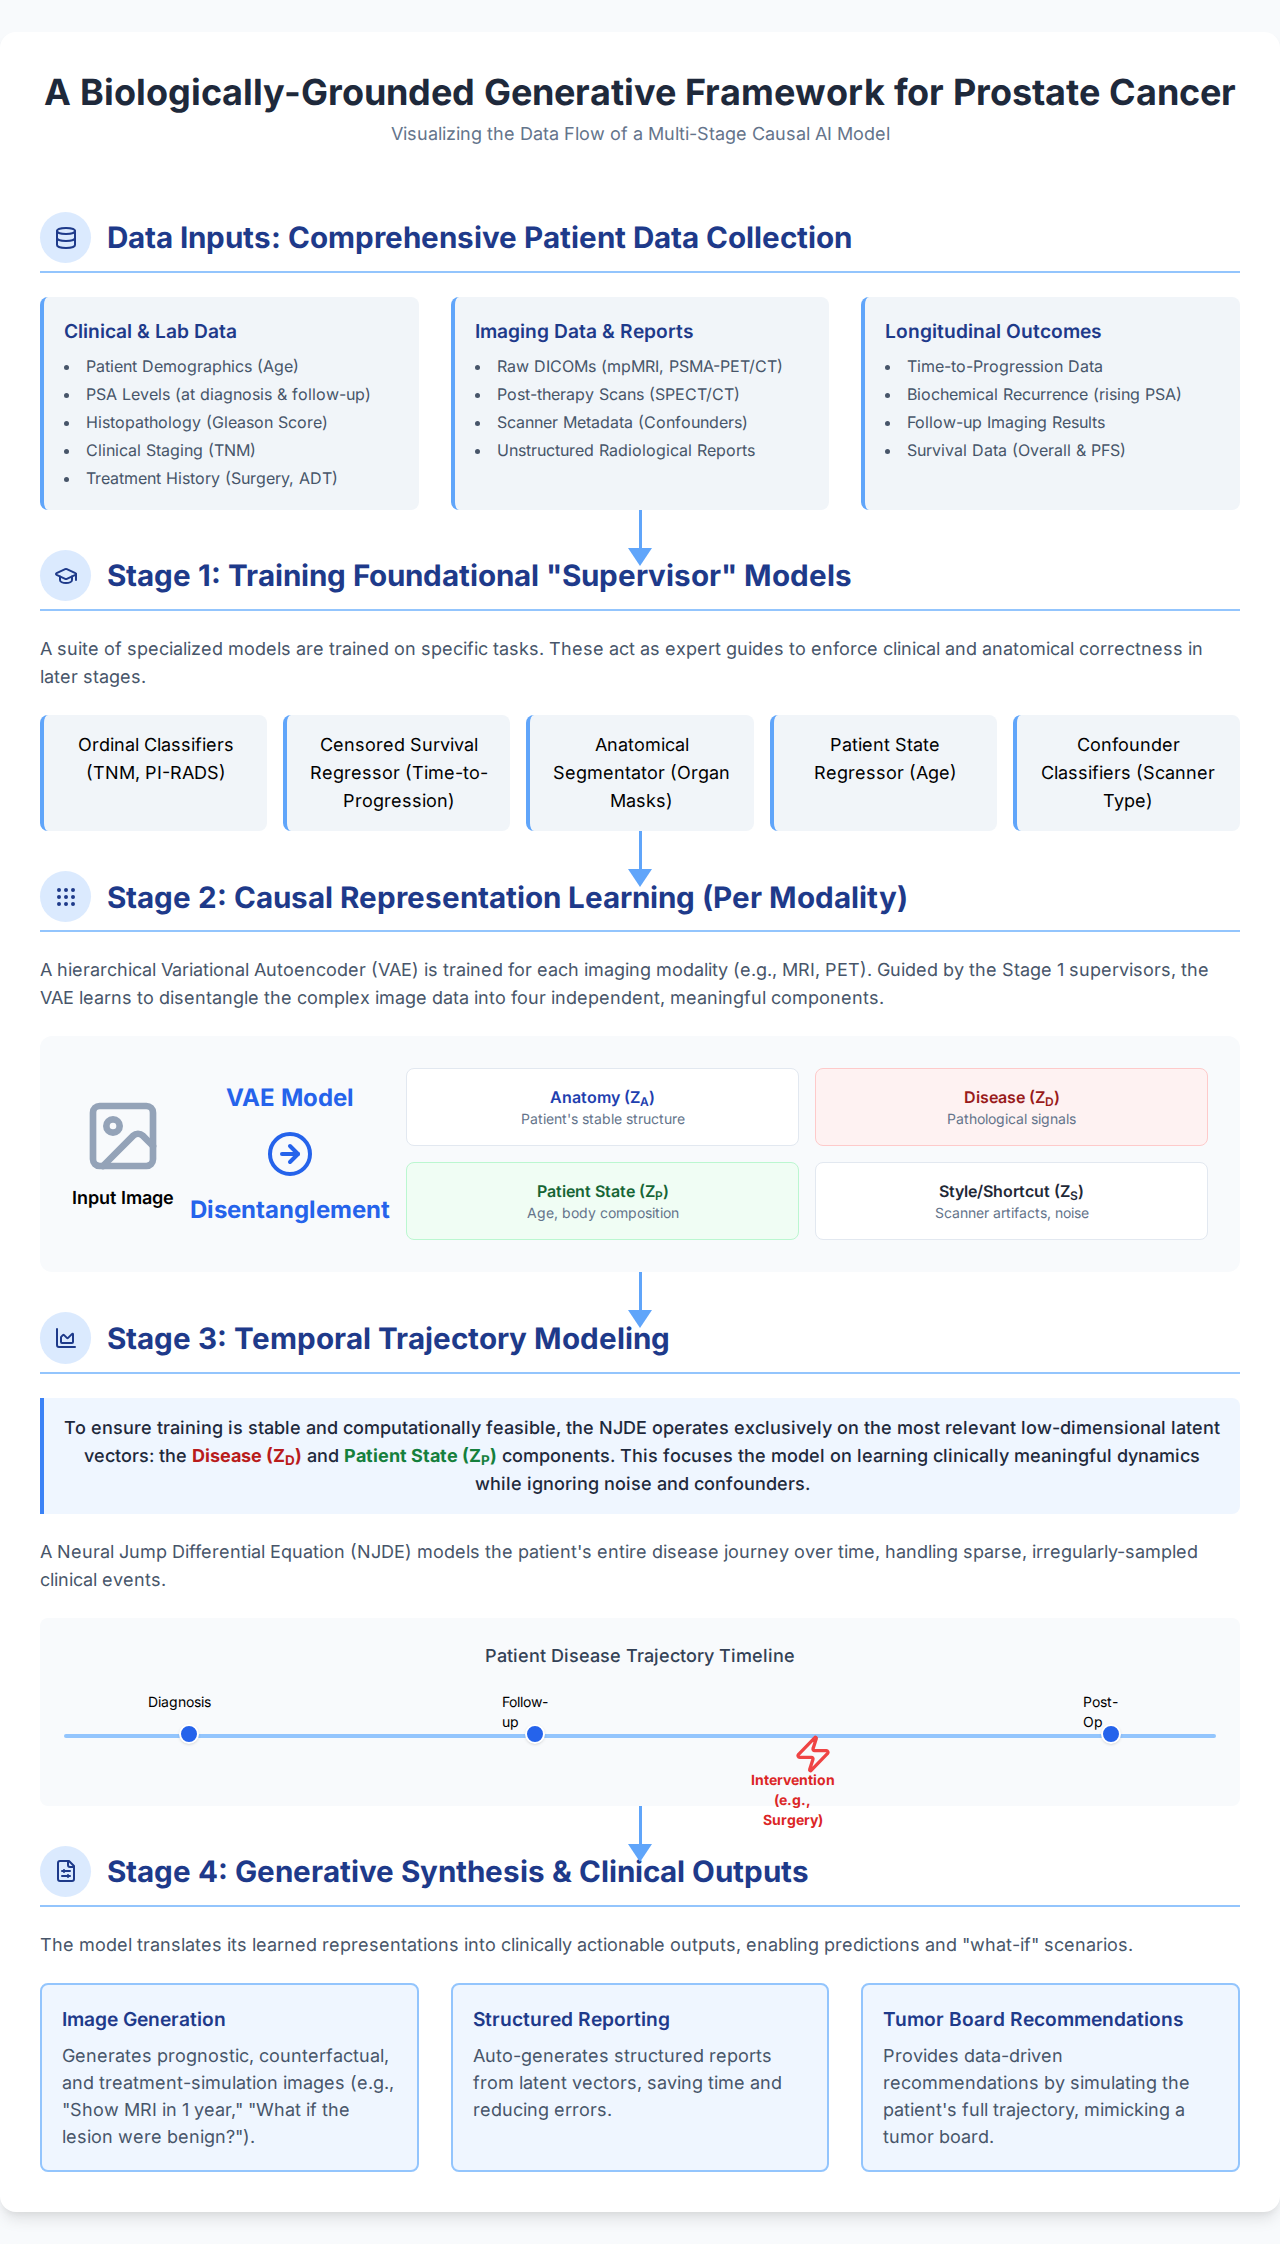
\includegraphics[width=1\textwidth]{ml.png}
    \caption{A high-level overview of the proposed multi-stage causal AI model, from data input to generative output.}
    \label{fig:ml_overview}
\end{figure}

\section{Work Plan}
The project is structured into seven Work Packages (WPs) spanning 36 months. WPs 1-4 represent the core technical development, building sequentially from data curation to the final temporal model. WP5 is dedicated to rigorous validation, while WPs 6 and 7 run for the project's duration, covering dissemination and management.

\subsection*{WP1: Data Curation (Months 1-9)}
\textbf{Objective:} To build a large-scale, high-quality, multi-center, and multimodal dataset that will serve as the foundation for the entire project.
\textbf{Tasks:}
\begin{itemize}
    \item T1.1: Finalize data sharing agreements and secure ethical approvals from all participating institutions.
    \item T1.2: Establish a secure, centralized XNAT repository for all incoming data.
    \item T1.3: Implement a non-destructive curation pipeline, including automated pseudonymization of all DICOM and clinical data.
    \item T1.4: Develop and apply standardized preprocessing protocols, including conversion of all imaging to NIFTI format and normalization of clinical parameters.
    \item T1.5: Utilize Natural Language Processing (NLP) tools to parse unstructured radiological reports and extract key structured information (e.g., PI-RADS scores, presence of metastases).
\end{itemize}
\textbf{Deliverable:} \textbf{D1.1} - Curated, version-controlled dataset with associated metadata (Month 9).

\subsection*{WP2: Foundational Supervisor Models (Months 4-15)}
\textbf{Objective:} To train a suite of specialized "supervisor" models that provide strong, clinically-validated signals to guide the main generative model.
\textbf{Tasks:}
\begin{itemize}
    \item T2.1: Train ordinal classifiers for clinical scores (TNM, PI-RADS, PSMA-RADS) using a differential ordinal learning framework.
    \item T2.2: Develop and train a censored survival regressor to predict time-to-progression, handling right-censored data appropriately.
    \item T2.3: Fine-tune and adapt a pre-trained anatomical segmentation model (e.g., TotalSegmentator) to provide a differentiable anatomical loss.
    \item T2.4: Train classifiers to identify technical confounders (e.g., scanner type, dosage) and patient state variables (e.g., age) to enable their disentanglement in WP3.
\end{itemize}
\textbf{Deliverable:} \textbf{D2.1} - A complete set of trained and validated supervisor models (Month 15).

\subsection*{WP3: Causal Variational Autoencoder (Months 10-24)}
\textbf{Objective:} To develop a per-modality generative model (VAE) that learns a disentangled latent space, separating causal biological factors from confounders.
\textbf{Tasks:}
\begin{itemize}
    \item T3.1: Implement the hierarchical VAE architecture with a composite loss function designed for staged training.
    \item T3.2: Conduct Phase 1 training, focusing on high-fidelity reconstruction and learning a stable representation of patient anatomy, guided by the anatomical segmentator.
    \item T3.3: Conduct Phase 2 training, focusing on generative control and explicit disentanglement. This involves using the WP2 supervisors to guide the model and penalizing total correlation between latent subspaces.
\end{itemize}
\textbf{Deliverable:} \textbf{D3.1} - A trained VAE model for each imaging modality, capable of disentangled representation and counterfactual generation (Month 24).

\subsection*{WP4: Temporal Trajectory Modeling (Months 18-30)}
\textbf{Objective:} To model the longitudinal dynamics of disease progression by learning from the sparse, irregular time-series of latent representations.
\textbf{Tasks:}
\begin{itemize}
    \item T4.1: Implement the Neural Jump Differential Equation (NJDE) framework.
    \item T4.2: Create a data structure of sparse, time-stamped latent state vectors for each patient, using the disease components (Z\textsubscript{D}) from the WP3 models.
    \item T4.3: Train the NJDE model using a masked loss function to learn both the continuous evolution of the disease and the discrete "jumps" caused by clinical interventions.
\end{itemize}
\textbf{Deliverable:} \textbf{D4.1} - A fully trained NJDE model capable of predicting patient-specific disease trajectories (Month 30).

\subsection*{WP5: Validation and Clinical Integration (Months 25-36)}
\textbf{Objective:} To rigorously validate the entire framework's performance, clinical plausibility, and potential for real-world workflow integration.
\textbf{Tasks:}
\begin{itemize}
    \item T5.1: Perform comprehensive quantitative evaluation of all model components using appropriate metrics (e.g., C-index, FID, Kappa).
    \item T5.2: Conduct a clinician-in-the-loop study where radiologists and oncologists score the clinical plausibility and explanatory usefulness of model-generated counterfactuals.
    \item T5.3: Run a comparative workflow study to measure the efficiency and accuracy gains achieved when clinicians use the system's automated structured reports versus traditional methods.
\end{itemize}
\textbf{Deliverable:} \textbf{D5.1} - A final validation report detailing the model's performance and clinical utility (Month 36).

\subsection*{WP6: Dissemination and Exploitation (Months 1-36)}
\textbf{Objective:} To ensure the project's results are shared widely with the scientific and clinical communities and to lay the groundwork for future exploitation.
\textbf{Tasks:}
\begin{itemize}
    \item T6.1: Publish findings in high-impact, peer-reviewed journals and present at major international conferences.
    \item T6.2: Create and maintain a project website and develop an open-source codebase for the framework.
    \item T6.3: Prepare and submit mid-term and final project reports.
\end{itemize}
\textbf{Deliverables:} \textbf{D6.1} - Mid-term Report (M18), \textbf{D6.2} - Final Scientific and Financial Report (M36).

\subsection*{WP7: Project Management (Months 1-36)}
\textbf{Objective:} To ensure the efficient coordination, administration, and financial management of the project.
\textbf{Tasks:}
\begin{itemize}
    \item T7.1: Coordinate all scientific and administrative activities between partners.
    \item T7.2: Monitor project progress, manage risks, and ensure timely delivery of milestones and deliverables.
    \item T7.3: Handle all financial aspects, including budget distribution and reporting to the funding agency.
\end{itemize}
\textbf{Deliverable:} Continuous management and reporting throughout the project's lifetime.

\begin{figure}[H]
    \centering
    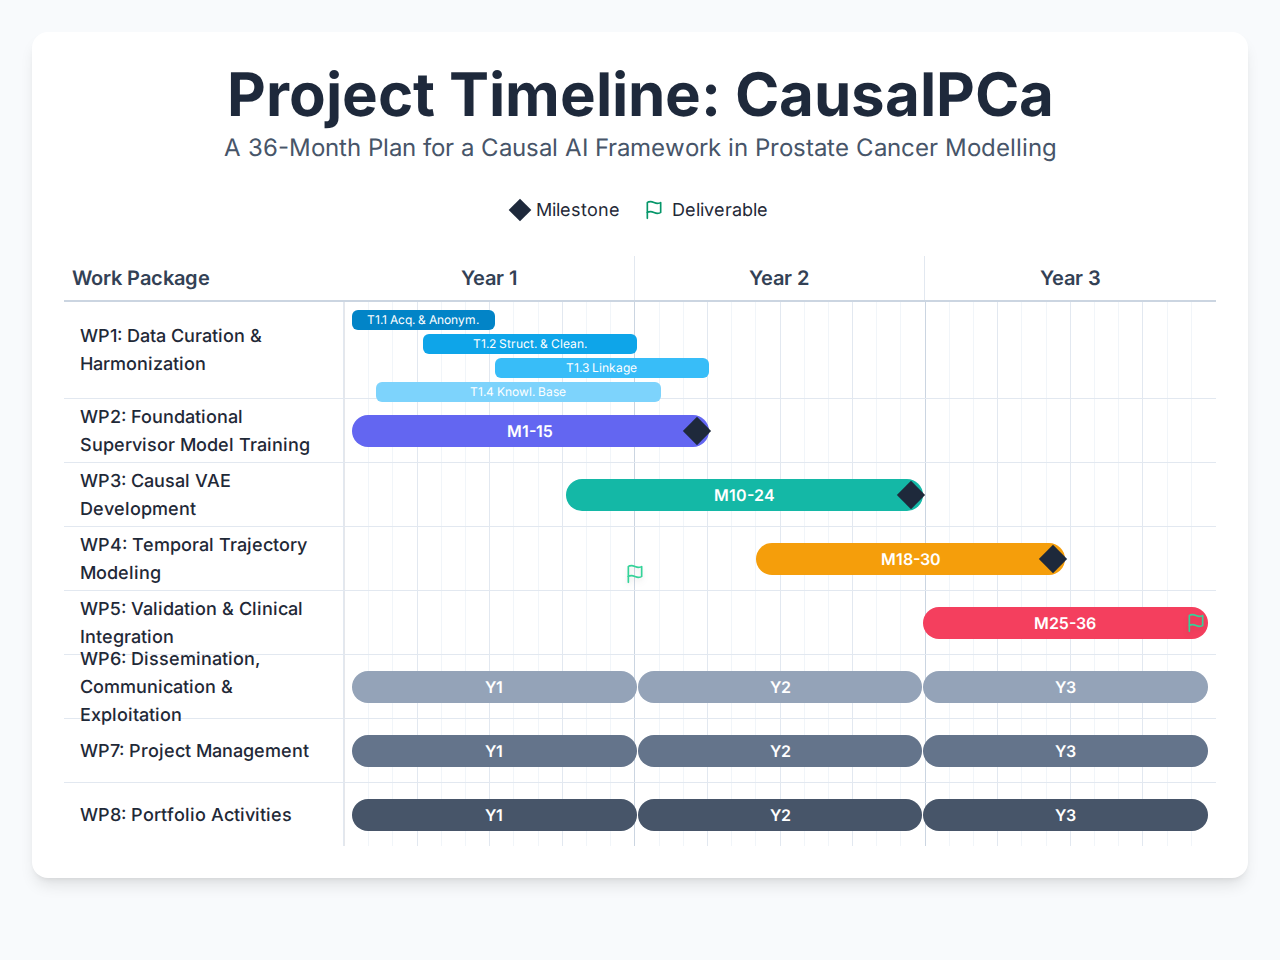
\includegraphics[width=1\textwidth]{gantt.png}
    \caption{Gantt chart outlining the project timeline and work packages over 36 months.}
    \label{fig:gantt_chart}
\end{figure}

Our vision is ambitious and high-risk, but the confluence of recent breakthroughs makes it achievable. Advances in generative modeling (VAEs, Diffusion Models), continuous-time dynamics (Neural ODEs), and the availability of rich, multimodal datasets, including from the innovative use of Lutetium-PSMA therapy, provide the necessary tools. This project will leverage these advances to create a foundational model for European oncology, with the potential for future integration into platforms like the European Cancer Imaging Initiative.

\begin{figure}[H]
    \centering
    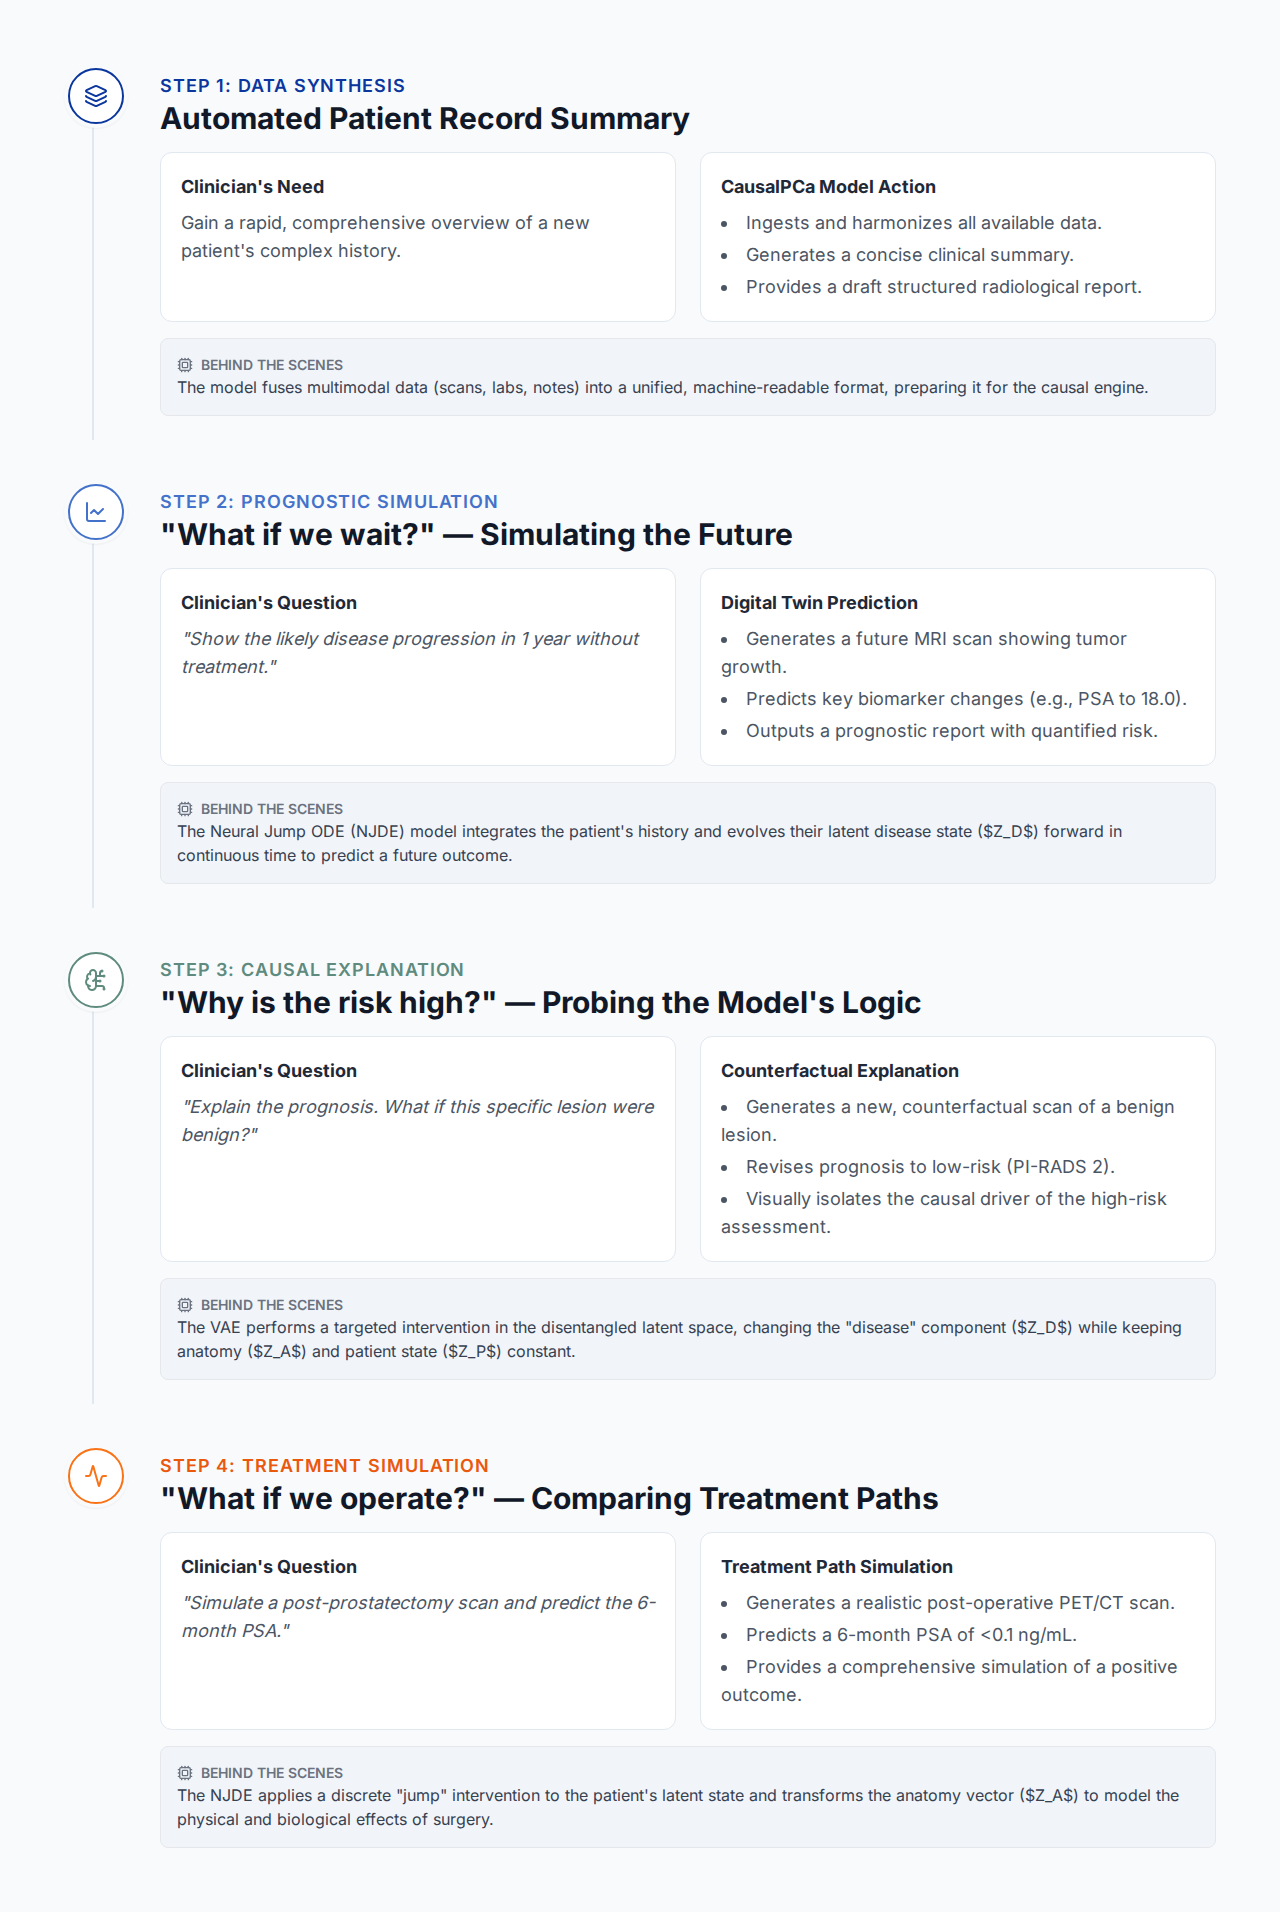
\includegraphics[width=1\textwidth]{wf.png}
    \caption{The Multidisciplinary Workflow of Prostate Cancer Diagnosis: A complex, iterative process requiring multimodal data fusion and expert collaboration.}
    \label{fig:workflow}
\end{figure}

\section{State of the Art and Project Objectives}

\subsection{Limitations of Current Predictive Models}
While the field of quantitative image analysis holds immense promise, its models are not yet universally proven to outperform classical clinical prediction models \cite{MolinBarry2024, FerroCobelli2022}. The process of extracting a large number of quantitative features from medical images, with the hypothesis that these features reflect underlying tumor biology \cite{MohseniniaZamaniSiahkali2024}, is hampered by significant methodological limitations. A primary challenge is the "curse of dimensionality," where the vast number of extracted quantitative features far exceeds the number of patients in a typical study. This creates a high risk of building models that are overfitted to the training data, capturing statistical noise rather than true biological signals, and severely limits their generalizability \cite{KendrickFrancis2021, GinsburgRsu2014}.

Deep learning models are prone to learning shortcuts from spurious correlations in the data rather than true causal relationships \cite{AydinHilbert2024, FayCobos2023}. For example, a model might link disease prediction to irrelevant factors like scanner type instead of the underlying pathology \cite{FayCobos2023, VigneshwaranOhara2024}. Generative models, such as VAEs, attempt to learn the underlying data-generating factors, but their latent representations often remain entangled, meaning a single latent factor influences multiple output features, which hampers interpretation and control \cite{CetinStephens2022}. Modeling disease evolution over time introduces further complexity, as clinical data is typically sampled irregularly, which does not reflect the continuous nature of a patient's biological evolution \cite{SeedatImrie2022, Purohit2023}.

\begin{figure}[H]
\centering
 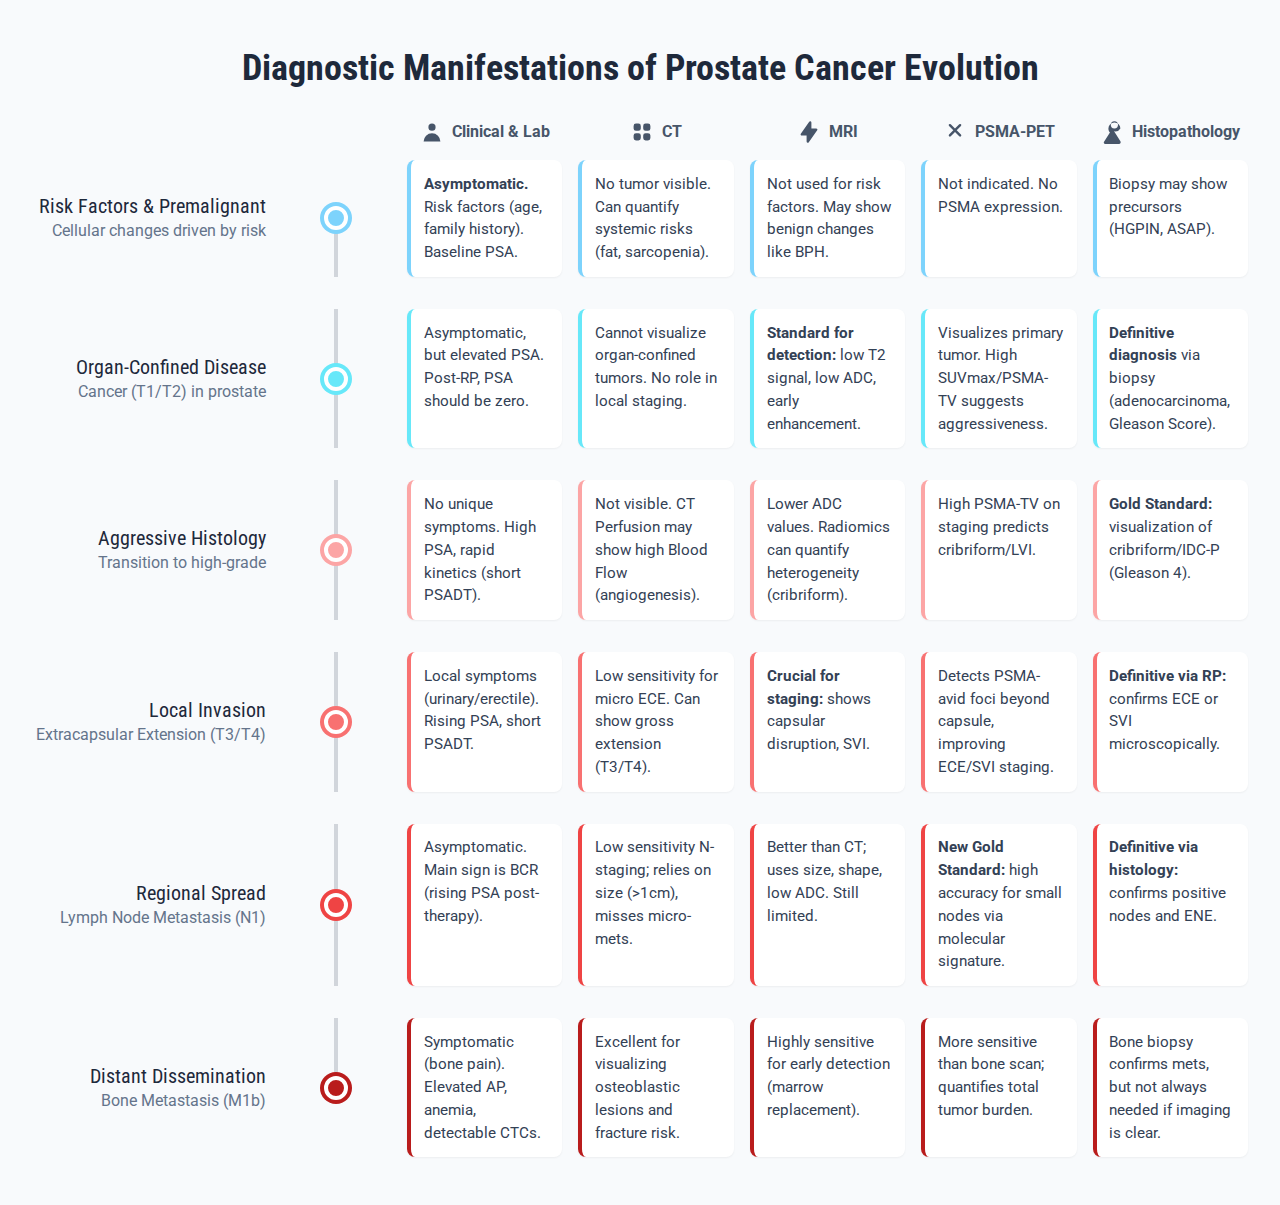
\includegraphics[width=\textwidth]{pe.png}
 \caption{An infographic illustrating the natural history of prostate cancer.}
\label{fig:prostate_evolution}
\end{figure}

\subsection{Project Objectives}
This project is a direct response to these limitations. Our goal is to develop a new generation of predictive models for prostate cancer that are causal, explainable, and robust to the challenges of real-world clinical data. The core objectives are:
\begin{enumerate}
    \item \textbf{Develop a Biologically-Grounded Generative Model:} To create a novel AI architecture based on a hierarchical Variational Autoencoder (VAE) that learns a disentangled representation of the disease. This model will explicitly separate anatomical structure, pathological signals, patient-specific characteristics, and technical confounders, guided by strong inductive biases from clinical domain knowledge.
    \item \textbf{Model Longitudinal Disease Trajectories:} To implement a Neural Jump Ordinary Differential Equation (NJDE) framework that operates on the learned latent space. This will allow us to model the continuous dynamics of disease progression from sparse, irregularly-sampled data while explicitly accounting for the discrete impact of clinical interventions like surgery or therapy.
    \item \textbf{Enable Causal and Counterfactual Reasoning:} To build a system capable of generating clinically plausible counterfactuals to explain its predictions. This will allow clinicians to ask "what-if" questions and simulate the outcomes of different treatment strategies, transforming the model from a "black box" into a transparent decision support tool.
    \item \textbf{Automate Clinical Reporting and Reduce Burden:} To leverage the model's disentangled representations to automatically generate accurate, consistent, and structured clinical reports, thereby streamlining the documentation process and improving data quality for research.
    \item \textbf{Validate in a Real-World Clinical Context:} To rigorously evaluate the model's performance, not only with quantitative metrics but also through a clinician-in-the-loop study assessing the clinical plausibility of its outputs and its impact on diagnostic workflow.
\end{enumerate}

\section{A Biologically-Grounded and Causal Approach}
To overcome the limitations of current "black-box" models, this project is founded on the principle of \textbf{biologically-grounded design}. Instead of allowing a neural network to learn arbitrary correlations from data, we embed strong inductive biases derived from clinical domain knowledge directly into the model's architecture. This ensures that the model learns representations that are not only predictive but also interpretable and aligned with the known pathophysiology of prostate cancer.

\subsection{Mimicking Clinical Reasoning via Disentanglement}
A radiologist does not interpret a scan as a collection of pixels; they first establish a baseline of the patient's unique anatomy and then identify how and where pathology deviates from that baseline. Our model's core architecture is designed to explicitly mimic this reasoning process. The hierarchical VAE (detailed in WP3) is tasked with disentangling the input image into independent latent subspaces:
\begin{itemize}
    \item \textbf{Anatomy ($Z_A$):} Represents the stable, patient-specific anatomical structure.
    \item \textbf{Disease ($Z_D$):} Represents the pathological signals corresponding to the cancer.
    \item \textbf{Patient State ($Z_P$):} Captures characteristics like age-related changes or body composition.
    \item \textbf{Style/Confounders ($Z_S$):} Isolates non-biological variations like scanner noise or protocol differences.
\end{itemize}
By forcing this separation, we ensure the model learns to distinguish what is patient, what is disease, and what is artifact. This allows for true counterfactual reasoning: we can ask the model to show what the patient's anatomy would look like \textit{without} the disease component, directly mirroring the diagnostic process.

\subsection{Modeling Disease as a Continuous Process with Discrete Interventions}
Prostate cancer evolution is not a series of disconnected snapshots. It is a continuous biological process, punctuated by discrete, transformative events like surgery, radiation, or the start of systemic therapy. Standard time-series models fail to capture this dual nature. Our choice of a \textbf{Neural Jump Differential Equation (NJDE)} framework (WP4) is a direct solution to this challenge.
\begin{itemize}
    \item The \textbf{continuous ODE component} learns the underlying differential equations governing tumor growth and change between clinical visits, robustly handling the irregular time intervals inherent to real-world data.
    \item The \textbf{discrete Jump component} explicitly models the instantaneous and profound impact of clinical interventions, allowing the model to learn the causal effect of a specific treatment on the disease trajectory.
\end{itemize}

\subsection{Respecting the Ordinality of Clinical Scores}
Clinical and pathological scoring systems like Gleason Score or PI-RADS are not arbitrary categories; they represent an ordered scale of biological aggressiveness and risk. Treating them as simple classes ignores this vital information. Our supervisor models (WP2) will be trained with \textbf{differential ordinal loss functions}. This forces the model to understand that misclassifying a PI-RADS 2 lesion as a 3 is a small error, while misclassifying it as a 5 is a major one. This embeds a fundamental aspect of clinical knowledge into the model's feature space, leading to more robust and clinically relevant representations.

\section{Methodology: A Multi-Stage Causal Framework}
To ensure stability and manage the complexity of multimodal data, the model is constructed using a sequential, multi-stage training framework. This approach decomposes the overall task into a series of manageable sub-problems, where each stage builds upon the foundations laid by the previous one. A visual overview of the proposed framework is presented in Figure \ref{fig:ml_framework}.

\begin{figure}[H]
    \centering
    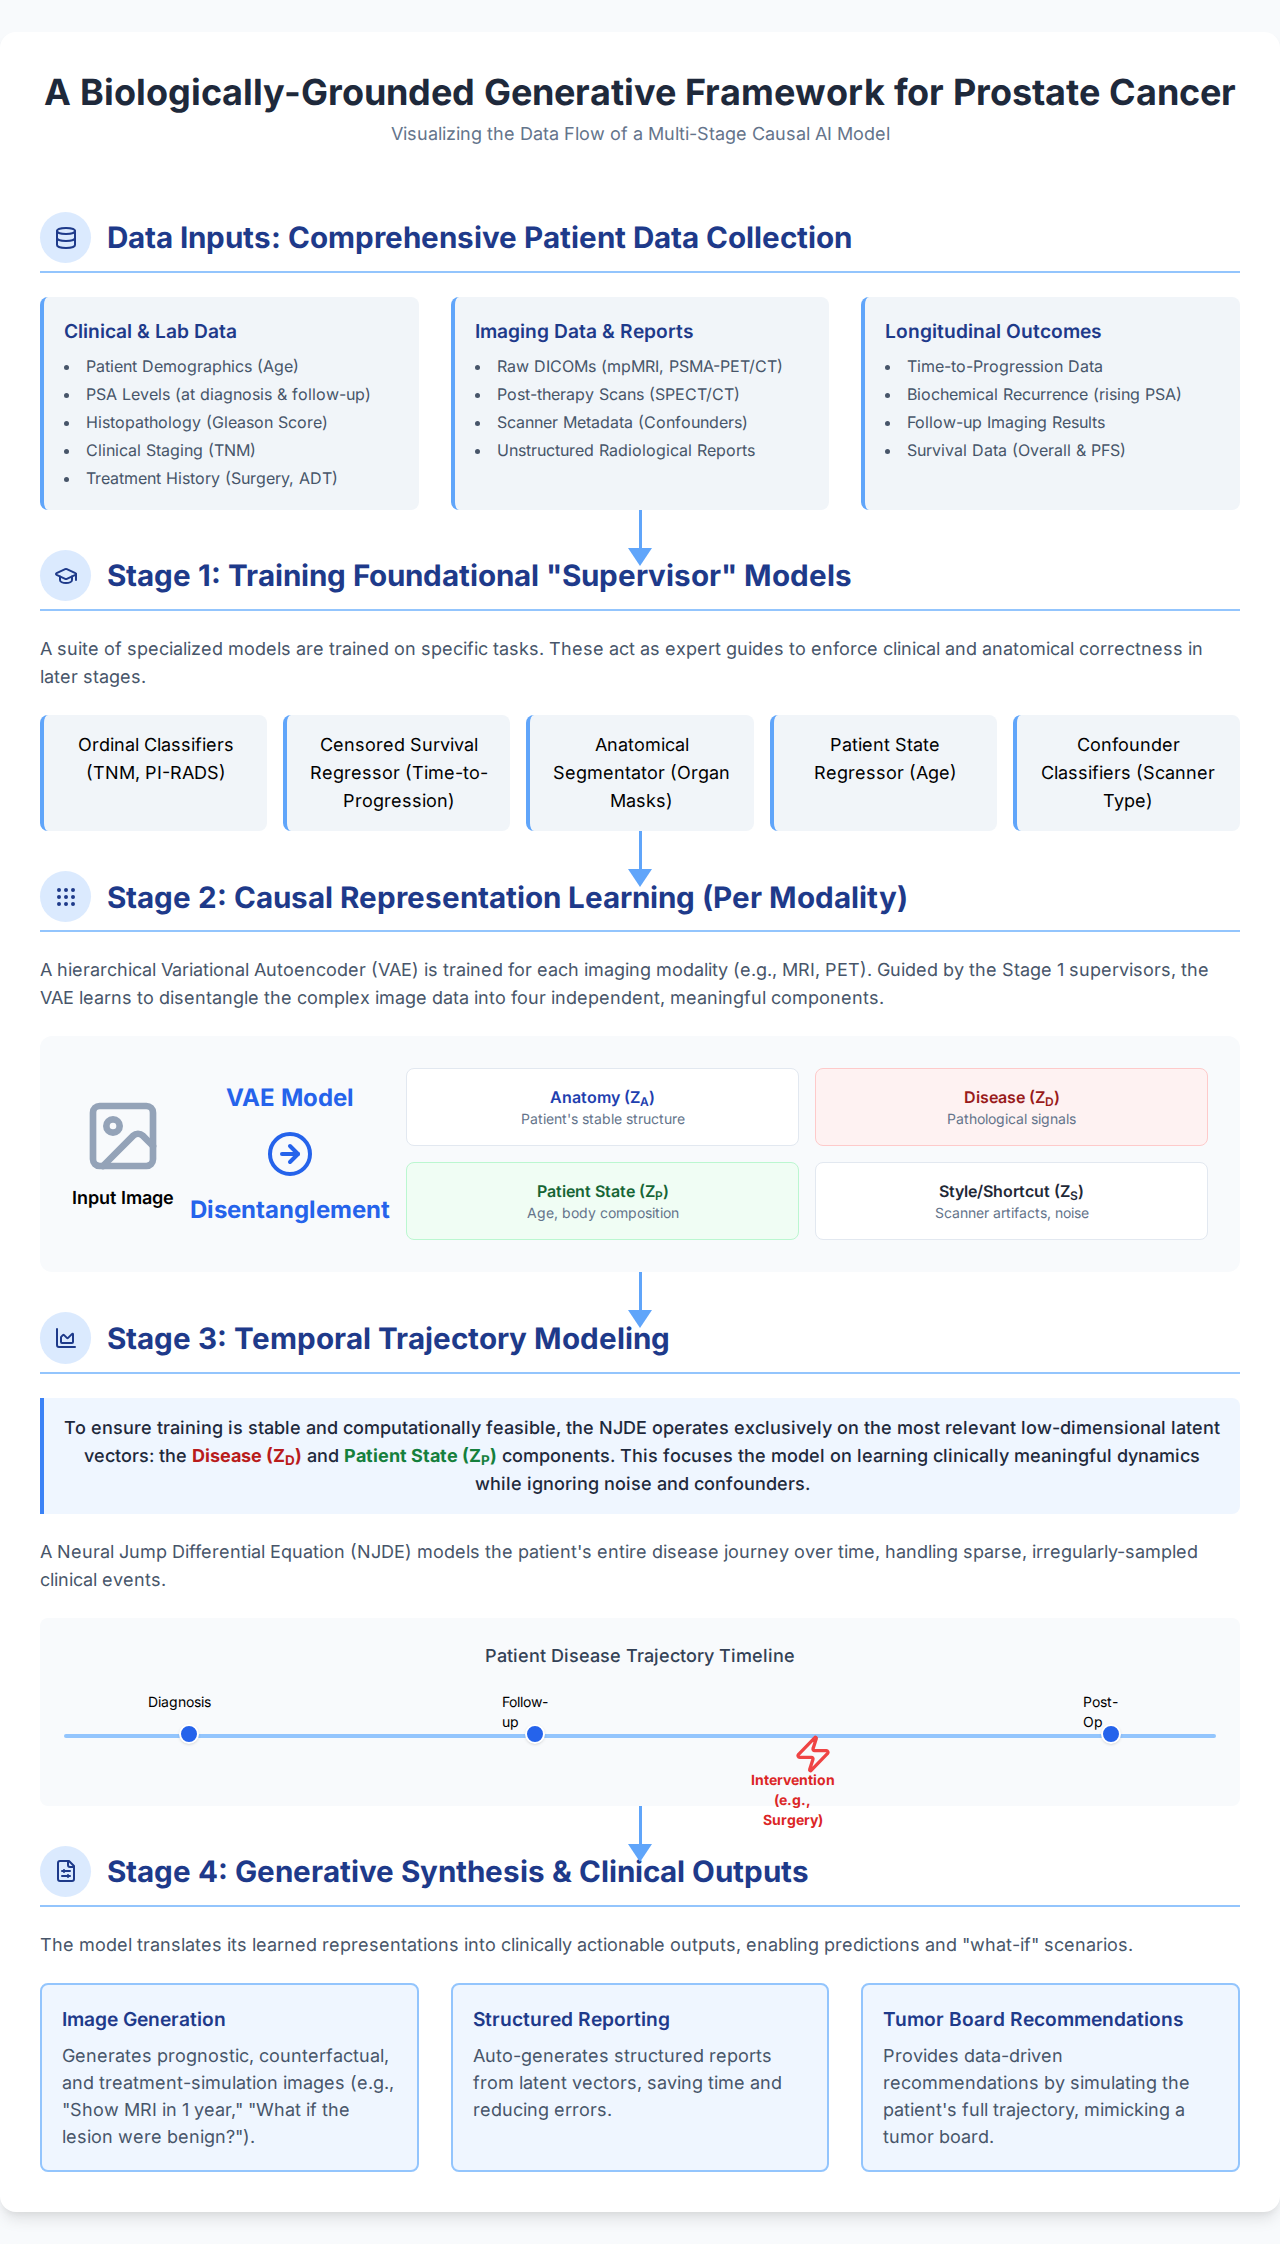
\includegraphics[width=\textwidth]{ml.png}
    \caption{The proposed multi-stage causal AI framework. Stage 1 trains supervisor models. Stage 2 learns disentangled representations with a VAE. Stage 3 models temporal dynamics with a Neural Jump ODE. Stage 4 generates clinical outputs.}
    \label{fig:ml_framework}
\end{figure}

\subsection{Stage 1: Training Foundational Supervisors}
The first stage involves training a suite of specialized "supervisor" models. These models act as expert guides, providing strong, accurate signals that will enforce a clinically valid structure on the more complex generative models in the subsequent stages. Each of these supervisors is based on established architectures and training paradigms for which practical implementation pathways have been demonstrated in the literature \cite{LeeByeon2025, GrisiKartasalo2025, RivailVogl2023, MehtaShui2023}.
\begin{itemize}
    \item \textbf{Ordinal Classifiers:} For clinical scores with an inherent order (e.g., PI-RADS, TNM stage), standard categorical classifiers using Cross-Entropy loss are suboptimal as they ignore the crucial ordering relationship (i.e., a higher grade implies a worse prognosis). To address this, we will train our classifiers using a more sophisticated \textbf{differential ordinal learning framework} \cite{LeeByeon2025}. This involves a multi-task approach where the model simultaneously learns to predict the specific class label and, critically, the degree of difference between pairs of samples, thus explicitly encoding the ordinal structure. The total loss function will be a hybrid, combining a standard categorical loss with a specialized differential ordinal loss (such as Negative Absolute Difference Log-likelihood), which is explicitly designed to handle ordered classes more effectively than conventional methods \cite{GrisiKartasalo2025}. These classifiers, built on Vision Transformer (ViT) backbones, will be trained for TNM Staging, PI-RADS (MRI), and PSMA-RADS/PROMISE (PSMA PET/CT).
    \item \textbf{Censored Survival Regressor:} To predict time to progression (TTP), we will train a survival model that properly handles right-censored data (e.g., patients with less than 6 months of follow-up who have not yet progressed). This will be achieved using a censored regression loss (e.g., Logistic Hazard or an Accelerated Failure Time log-likelihood loss) combined with a ranking loss regularizer (e.g., SurvRNC) to ensure correct risk ordering in the learned feature representation \cite{GaoLi2019, RivailVogl2023, ShahinZhao2023, SaeedRidzuan2024, ApellnizParras2024}.
    \item \textbf{Anatomical Segmentator:} A pre-trained TotalSegmentator model will be fine-tuned to generate gold-standard anatomical segmentations. A version will be adapted to operate directly on tensors, providing a differentiable anatomical loss for the VAE training.
    \item \textbf{Patient State Regressor (Age):} As age is a critical risk factor and also drives benign anatomical changes, we will train a dedicated regressor to predict patient age from imaging. This allows us to explicitly model and control for age-related effects, separating them from pathology \cite{PuglisiAlexander2025, ZhangHager2025}.
    \item \textbf{Technical Confounder Classifiers:} To isolate non-clinical sources of variation, we will train classifiers for: scanner type, PSMA/Lutetium dosage, and patient BMI.
\end{itemize}

\subsection{Stage 2: Per-Modality Causal Representation Learning}
For each imaging modality $m$, we train a separate hierarchical Variational Autoencoder (VAE), likely based on an efficient 3D Vision Transformer (ViT) or 3D CNN backbone, to learn a disentangled latent space, $Z_m$ \cite{KimOh2025, LeeByeon2025, FragemannArdizzone2022}. The VAE compresses a high-dimensional image $x_m$ into a low-dimensional summary (the latent space) and then reconstructs it \cite{HeSarwal2024, FriedrichFrisch2024}. The key innovation is that this latent space is partitioned into independent, semantically meaningful components:
$$ Z_m = Z_A \oplus Z_D \oplus Z_P \oplus Z_S $$
Here, $\oplus$ denotes concatenation, and the components represent \textbf{Anatomy} ($Z_A$), \textbf{Disease} ($Z_D$), \textbf{Patient State} (age-related changes, $Z_P$), and \textbf{Style/Shortcut} (technical artifacts, $Z_S$). This separation is enforced through a complex, multi-stage training process governed by a composite loss function that leverages the supervisors from Stage 1.

\subsubsection{Composite Loss Function and Staged Training}
The training is carefully staged to ensure stability and guide the VAE towards the correct solution. The total loss, $\mathcal{L}_{\text{total}}$, is a weighted sum of several components:
$$ \mathcal{L}_{\text{total}} = \mathcal{L}_{\text{VAE}} + \lambda_A \mathcal{L}_{\text{Anatomy}} + \lambda_D \mathcal{L}_{\text{Disease}} + \lambda_I \mathcal{L}_{\text{Disentangle}} $$
The core VAE loss, $\mathcal{L}_{\text{VAE}}$, consists of a reconstruction term and a Kullback-Leibler (KL) divergence term, $D_{KL}(q_{\phi}(Z|X)||p(Z))$, which regularizes the learned latent space. The training proceeds as follows:
\begin{enumerate}
    \item \textbf{Anatomy and Identity Pre-training (e.g., first 100 epochs):} The initial phase focuses on learning stable representations of anatomy and achieving high-fidelity reconstruction.
    \begin{itemize}
        \item \textbf{Anatomy Consistency ($\mathcal{L}_{\text{Anatomy}}$):} A synthetic image generated purely from the anatomy component ($Z_A$) is penalized if its segmentation (from the pre-trained TotalSegmentator) does not match the ground truth. Registration-guided consistency is also enforced, ensuring that elastic deformations applied to the input image result in corresponding deformations in the latent space \cite{LiChen2024}.
        \item \textbf{Healthy State Enforcement:} The image generated from $Z_A$ is passed to the disease classifiers from Stage 1, and the loss function penalizes any classification other than "healthy."
        \item \textbf{Identity Transformation:} To begin, the disease component ($Z_D$) is trained for identity transformation. The full reconstructed image (from $Z_A$ and $Z_D$) is supervised to match the original image's clinical labels (TNM, PI-RADS, etc.) using the Stage 1 classifiers. Standard reconstruction losses like L1 and multi-scale structural similarity are dominant here \cite{FerreiraLi2024, KhojasteSarakhsiHaghighi2024}.
    \end{itemize}
    \item \textbf{Generative and Disentanglement Training:} After the VAE has learned a stable anatomical basis, the training shifts to generative control and explicit disentanglement.
    \begin{itemize}
        \item \textbf{Generative Disease Control ($\mathcal{L}_{\text{Disease}}$):} The VAE is now tasked with a more complex goal. It receives a random target class (e.g., "PI-RADS 5" or "TNM Stage 3") and must modify the image generated from the anatomy component ($Z_A$) using the disease component ($Z_D$) such that the final image is correctly classified as the target class by the corresponding supervisor.
        \item \textbf{Explicit Disentanglement ($\mathcal{L}_{\text{Disentangle}}$):} The implicit regularization from the standard VAE's KL-divergence term is insufficient for robust disentanglement. Simply increasing its weight (as in a $\beta$-VAE) can degrade reconstruction quality by excessively penalizing the mutual information between the input and the latent space \cite{FragemannArdizzone2022, CetinStephens2022}. Our approach is more targeted. The KL-divergence term can be decomposed to isolate the \textbf{Total Correlation (TC)}, which specifically measures the statistical dependence among the individual latent dimensions \cite{FragemannArdizzone2022, AbbasiMonadjemi2018}. Our disentanglement loss, $\mathcal{L}_{\text{Disentangle}}$, will therefore heavily penalize the TC term, forcing the latent subspaces to become independent without sacrificing the information content needed for high-quality image generation. Furthermore, we will explicitly minimize the mutual information between specific subspaces that are causally independent, such as between the disease ($Z_D$) and style ($Z_S$) components, to ensure the learned disease representation is invariant to scanner-specific artifacts \cite{FayCobos2023}.
    \end{itemize}
\end{enumerate}

\subsection{Stage 3: Temporal Trajectory Modeling with Neural Jump ODEs}
This stage addresses the critical challenge of modeling disease evolution from sparse, multimodal, and irregularly-sampled clinical data. Our solution is a \textbf{Neural Jump Differential Equation (NJDE)} framework, which is uniquely suited for this task \cite{GwakSim2020}.

\subsubsection{Rationale and Latent State Formulation}
Neural Ordinary Differential Equations (NODEs) are powerful because they model system dynamics in continuous time, making them inherently robust to irregular sampling—a defining characteristic of clinical data \cite{GwakSim2020, JohnsonBulgarelli2023, BelogolovskyGreenberg2023}. However, their primary weakness is the extreme computational cost of applying them directly to high-dimensional data like 3D images \cite{WiewelBecher2018, DavisChoromanski2020}. Our approach strategically mitigates this by operating exclusively on the low-dimensional latent spaces learned in Stage 2. This is not just an efficiency gain; by training the NODE only on the disentangled \textbf{disease part of the latent space ($Z_D$)}, we focus the model on learning the dynamics of disease progression itself, making the learning task more tractable and clinically relevant \cite{AshmanSo2020, KberKalisch2023, LosadaTerranova2024}.

The input for the NJDE is a carefully constructed time series of latent state vectors. For each patient, we define a unified state vector $\mathbf{v}$ that has a fixed shape, representing a concatenation of all possible inputs. The process is as follows:
\begin{enumerate}
    \item \textbf{Unified State Vector Definition:} A canonical tensor shape is defined for a state vector $\mathbf{v}$, which includes dedicated slots for the disease latent code ($Z_D$) from each imaging modality (MRI, PET, SPECT) and for embeddings of all non-imaging data (PSA, clinical note embeddings, etc.).
    \item \textbf{Time-stamped Sparse Tensor Creation:} For each time point $t_i$ where a patient has data, a new state vector $\mathbf{v}(t_i)$ is created and initialized with zeros. The available data is then placed into its corresponding slot in the tensor. For example, at a time point with a PET scan and PSA value, only the $Z_{D_{\text{PET}}}$ and PSA embedding slots are filled, while all other slots (for MRI, notes, etc.) remain zero.
    \item \textbf{Anatomy Vector Storage:} The patient-specific anatomy vectors ($Z_A$) from each imaging study are not included in the dynamic state vector but are stored separately, indexed by time, for use in the final image reconstruction stage.
\end{enumerate}
This procedure yields a dataset of sparse, irregularly-sampled latent state vectors, providing a computationally efficient and robust representation of each patient's unique clinical history.

\subsubsection{NJDE Training and Dynamics}
The NJDE learns the rules of disease evolution by modeling two phenomena \cite{GwakSim2020}:
\begin{itemize}
    \item \textbf{Continuous Evolution (The NODE):} Between clinical events, the disease state evolves smoothly. This is modeled by a classic NODE that learns the underlying dynamics from the sparse state vectors \cite{BergHasenclever2018}.
    $$ \frac{d\mathbf{v}(t)}{dt} = f(\mathbf{v}(t), t; \psi) \quad \text{for } t \neq t_k $$
    \item \textbf{Discrete Jumps (The Interventions):} At the specific time $t_k$ of a clinical intervention (e.g., prostatectomy, initiation of hormonal therapy), the continuous evolution is interrupted by a discrete "jump." A separate neural network, $g$, models this instantaneous change to the state vector based on the type of intervention \cite{CuchieroLarsson2019, AbushaqraXue2022}.
    $$ \mathbf{v}^+ = g(\mathbf{v}(t_k), \text{intervention}_k; \phi) \quad \text{for } t = t_k $$
\end{itemize}
This hybrid approach, which explicitly separates the continuous disease course from the rapid, external impacts of clinical interventions, is critical for accurately modeling a patient's journey \cite{GwakSim2020}. The model is trained using a leave-one-out strategy for each patient's time series: given all but one time point, its goal is to predict the complete state vector for the held-out time point. To handle the pervasive missing data, we employ a \textbf{masked loss function}. The loss is calculated only by comparing the predicted values to the ground truth for those elements of the state vector that were actually available (non-zero) at the target time point. This forces the model to learn a probable evolution for every data type, even from a highly incomplete dataset.

\subsection{Stage 4: Generative Synthesis and Clinical Outputs}
The final stage translates the model's internal representations back into clinically useful outputs, including high-fidelity images and actionable, structured text.

\subsubsection{Image Generation and Refinement}
A final image for any time point (past, present, or future) and for any modality is generated by combining the appropriate anatomy vector ($Z_A$) with the disease vector ($Z_D$) predicted by the NJDE. An additional model is trained on the anatomy vectors to simulate post-prostatectomy changes. To ensure clinical realism, the generated VAE image is passed through a lightweight Diffusion Model that acts as a post-processor, adding high-frequency textural details and sharpness.

\subsubsection{Structured Report and Recommendation Generation}
A key output of our framework is the generation of structured reports, which are critical for enhancing clinical quality, standardization, and efficiency \cite{JorgHalfmann2023}. Structured reports are more complete, reduce errors, and provide data that is immediately usable for AI training and research \cite{SacoranskyKwan2024}. Our system will produce two types of structured text outputs using a Transformer-based decoder:
\begin{itemize}
    \item \textbf{Structured Radiological Reports:} For any imaging study (real or counterfactual), the decoder will take the corresponding anatomy ($Z_A$), disease ($Z_D$), and patient state ($Z_P$) latent vectors as input. It will generate a report that follows a predefined schema (e.g., a Pydantic model) composed primarily of closed questions and standardized fields. A section for supplementary free-text narrative will be included, but this part will be ignored in subsequent modeling steps to enhance system robustness. This unique link to the latent space allows the model to generate a descriptive report not just for an existing scan, but also for a counterfactual one (e.g., "Describe the MRI if the patient were 10 years older.").
    \item \textbf{Tumor Board Recommendations:} The NJDE, by modeling both continuous progression and discrete treatment \textit{jumps}, produces a comprehensive, dynamic model of the entire patient trajectory. A separate generative module will take this complete trajectory as input—synthesizing all available information across all time points. Based on this history and the model's prediction of the future disease course, it will generate a structured report with recommendations for further patient management, effectively simulating a data-driven tumor board consultation.
\end{itemize}

\section{Data Sources and Cohort}
The project will leverage a unique combination of proprietary, multi-center clinical data and large-scale public datasets. This hybrid approach ensures that our models are trained on a rich, diverse, and clinically relevant cohort, while also being validated against established international benchmarks to ensure generalizability.

\subsection{Proprietary Multi-Center Clinical Cohort}
A key strength of this proposal is the direct access to rich, longitudinal, and multimodal data from the applicants' own clinical institutions and established collaborators. This will form the core training dataset.

\begin{itemize}
    \item \textbf{Universitätsklinik für Radiologie und Nuklearmedizin (Magdeburg):} As the lead applicant institution, the clinic will provide a rich dataset from its patient care archives. This includes:
    \begin{itemize}
        \item Approximately 100 longitudinal studies of patients with paired baseline PSMA-PET/CT and mpMRI scans for primary staging and follow-up.
        \item A unique cohort of approximately 100 patients with advanced disease who have undergone Lutetium-177 PSMA radioligand therapy (RLT). For these patients, we have paired pre-therapy PSMA-PET/CT scans and post-therapy Lutetium SPECT/CT scans, which are essential for modeling treatment response.
    \end{itemize}
    \item \textbf{Abteilung für Nuklearmedizin | Universitätsmedizin Halle:} This collaborating institution will provide a comparable dataset, enriching the cohort's geographical and technical diversity. It is expected to contribute:
    \begin{itemize}
        \item Approximately 100 additional paired PSMA-PET/CT and mpMRI studies.
        \item Approximately 100 additional paired pre-therapy PSMA-PET/CT and post-therapy Lutetium SPECT/CT studies.
    \end{itemize}
    \item \textbf{Private Practice of Christian Wybrański (Magdeburg):} This collaboration provides access to a significant number of high-quality diagnostic scans from a private practice setting, further enhancing the dataset's diversity.
    \begin{itemize}
        \item Approximately 200 paired mpMRI studies for diagnosis and active surveillance.
    \end{itemize}
\end{itemize}
This combined proprietary cohort of over 500 patients, with its unique inclusion of post-RLT SPECT/CT data, provides an unparalleled resource for training a model capable of understanding the entire spectrum of prostate cancer progression and treatment.

\subsection{Integration with Public Datasets}
To augment our proprietary data, enhance statistical power, and rigorously test the generalizability of our models, we will integrate several large, well-curated public datasets. These have been chosen to cover a wide range of clinical scenarios, imaging modalities, and patient populations.
\begin{itemize}
    \item \textbf{The Cancer Genome Atlas Prostate Adenocarcinoma (TCGA-PRAD):} This will serve as a primary resource for linking our imaging-based models to underlying genomic data. Its rich, multi-modal imaging (MRI, CT, PET) and detailed clinical and genomic information are ideal for validating our model's biological grounding.
    \item \textbf{ProstateNET (EUCAIM):} Specifically, we will leverage the UC8 dataset for active surveillance, which contains longitudinal MRI and PSA data. This aligns with the European Union's goal of fostering a shared cancer imaging infrastructure.
    \item \textbf{NAF-PROSTATE:} This dataset provides systematic longitudinal PET/CT data for patients with bone metastases, which will be invaluable for validating the temporal modeling of our framework (WP4) in an advanced disease setting.
\end{itemize}

\begin{figure}[H]
        \centering
        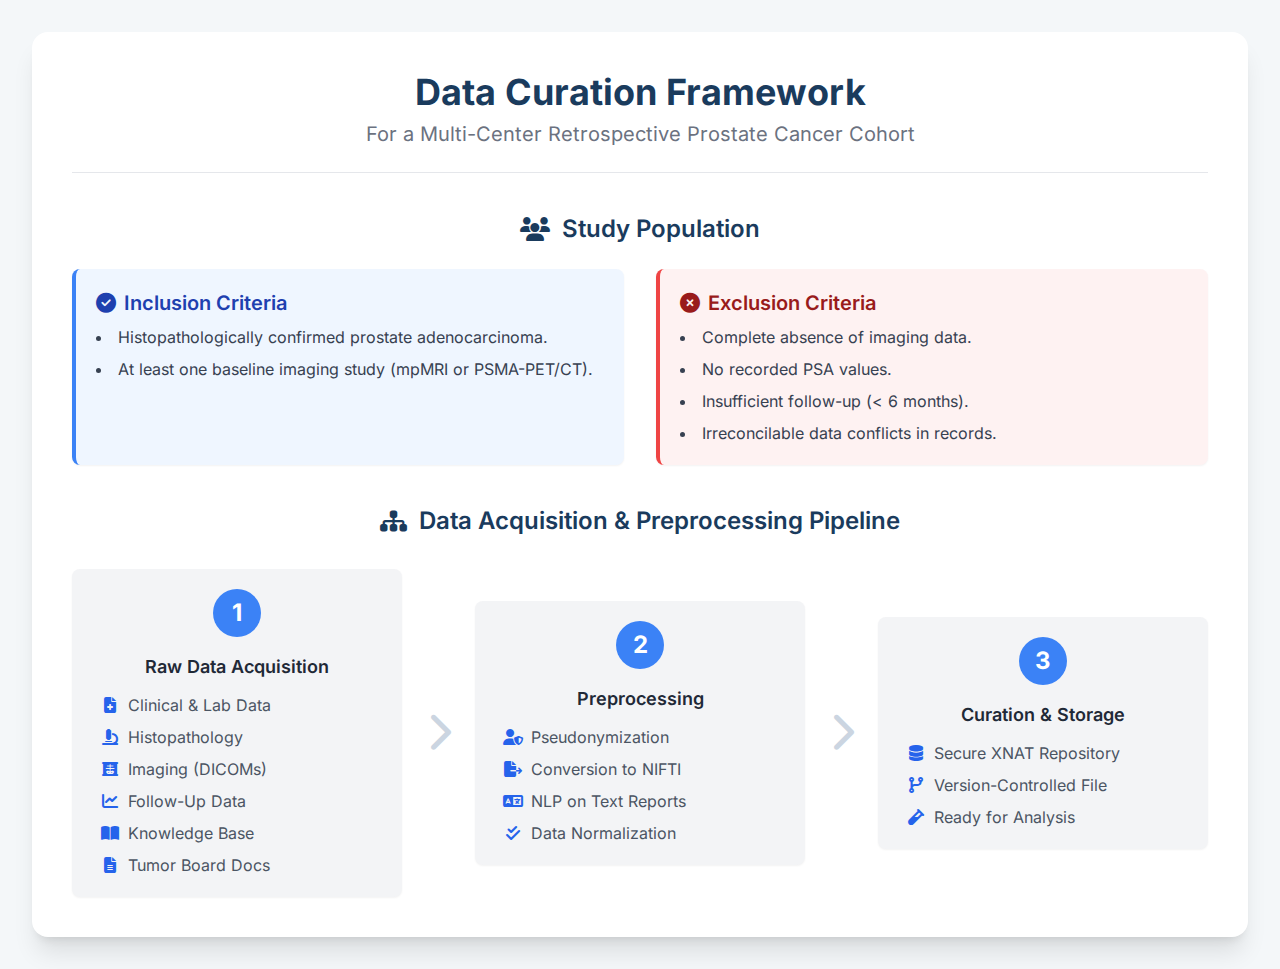
\includegraphics[width=\textwidth]{dc.png}
        \caption{An infographic summarizing the data acquisition, curation, and preprocessing framework for the study cohort. It details the inclusion and exclusion criteria for patient selection and outlines the multi-step pipeline for processing clinical, histopathological, and imaging data.}
        \label{fig:data_curation}
\end{figure}

\subsection{Consortium and Expertise}
The success of this high-risk, high-gain project hinges on a consortium with deep, interdisciplinary expertise. The applying institution, the Universitätsklinik für Radiologie und Nuklearmedizin, is uniquely positioned to lead this effort.
\begin{itemize}
    \item \textbf{Clinical and AI Leadership:} The project requires a leader with dual expertise in medicine/diagnostics and artificial intelligence. The clinic has an established leader with this exact profile, ensuring seamless integration of clinical needs and technical development.
    \item \textbf{Proven Track Record in Generative AI:} The clinic has prior experience in developing and applying generative models, including the synthesis of CT images from PET data.
    \item \textbf{Experience in Multimodal Modeling:} The team has a track record of creating models that predict disease progression by fusing clinical and imaging data.
    \item \textbf{Expertise in Structured Reporting and NLP:} The clinic has developed applications using structured reporting and has built an LLM-based support app for thyroid cancer guidelines, demonstrating proficiency in both creating structured data and processing unstructured text.
\end{itemize}
This unique combination of a rich, proprietary dataset and a team with a proven track record in all the core technical areas of this proposal significantly mitigates the project's risks and provides a strong foundation for its success.

\section{Work Plan and Timeline}
The project will be executed over a 36-month period, organized into six work packages (WPs). A detailed Gantt chart is provided in a separate HTML file.

\begin{itemize}
    \item \textbf{WP1: Project Management and Ethical Approval (Months 1-3):} Finalize consortium agreements, establish project governance, and secure all necessary ethical approvals for data sharing.
    \item \textbf{WP2: Data Collection, Curation, and Harmonization (Months 2-9):} Collect data from all partner sites, perform pseudonymization, and implement the standardized curation and preprocessing pipeline.
    \item \textbf{WP3: Foundational Supervisor Model Training (Months 6-15):} Develop and validate the suite of supervisor models (Ordinal Classifiers, Survival Regressor, etc.) that will guide the main generative model.
    \item \textbf{WP4: Causal Representation Learning (Months 12-24):} Train and validate the hierarchical VAE for each imaging modality to learn the disentangled latent spaces. This is the most research-intensive phase.
    \item \textbf{WP5: Temporal Trajectory Modeling (Months 20-30):} Develop and train the Neural Jump ODE model on the latent time-series data to model disease progression and treatment effects.
    \item \textbf{WP6: Integration, Evaluation, and Dissemination (Months 28-36):} Integrate all components into a final demonstrator, conduct the clinical workflow evaluation study, and disseminate the results through publications and conference presentations.
\end{itemize}

\begin{figure}[H]
    \centering
    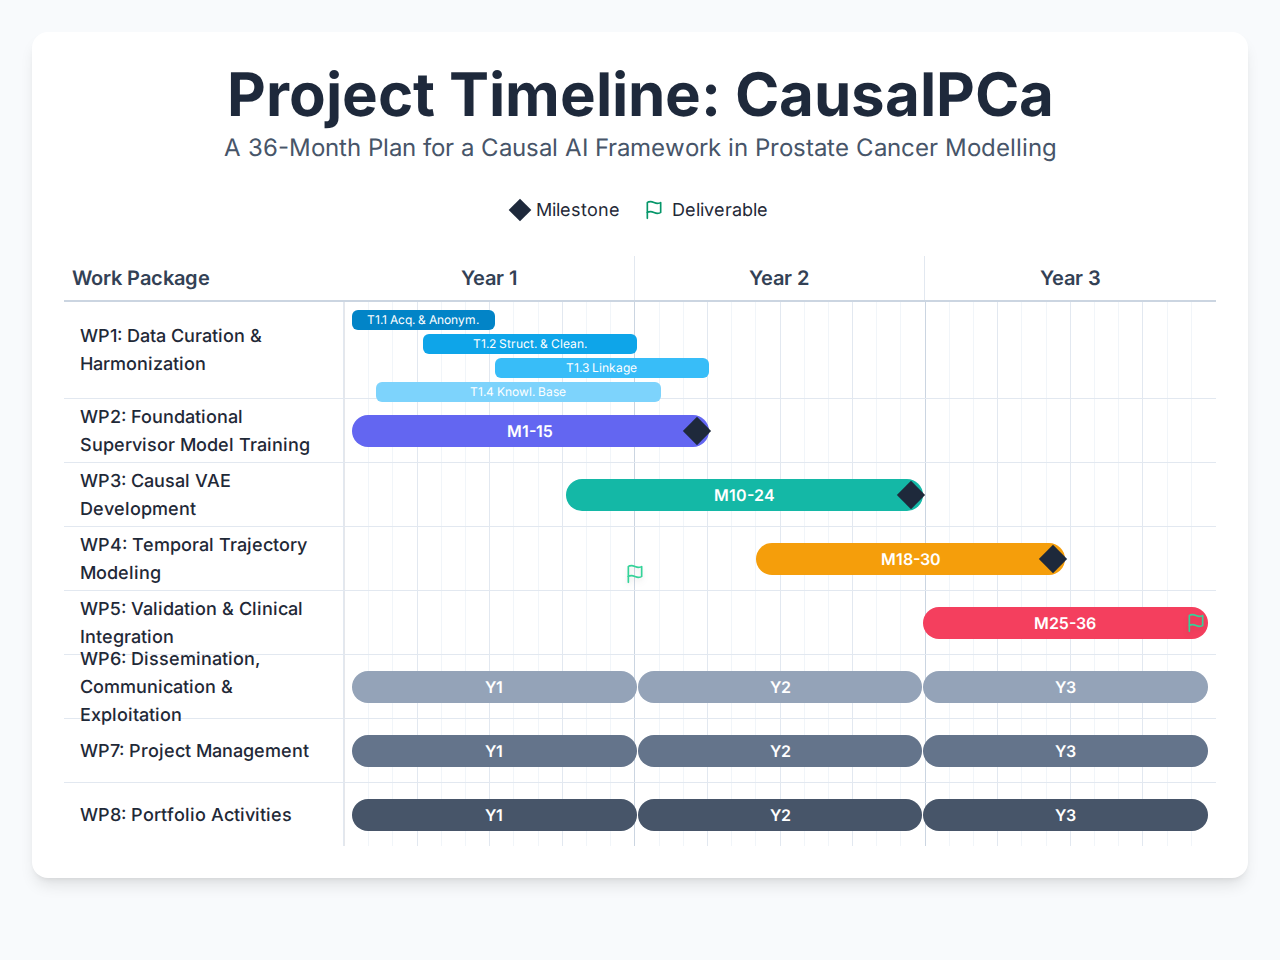
\includegraphics[width=\textwidth]{gantt.html}
    \caption{A Gantt chart illustrating the project's work plan and timeline.}
    \label{fig:gantt}
\end{figure}

\section{Evaluation and Impact}
\subsection{Evaluation}
Model performance will be rigorously assessed using a comprehensive suite of metrics tailored to each sub-task.
\begin{itemize}
    \item \textbf{Classification:} Accuracy, Area Under the Curve (AUC), F1-Score, and Quadratic Weighted Kappa (for ordinal tasks).
    \item \textbf{Survival Regression:} Concordance Index (C-index) and Mean Absolute Error on censored data.
    \item \textbf{Image Generation:} Fréchet Inception Distance (FID), Structural Similarity Index (SSIM), and Learned Perceptual Image Patch Similarity (LPIPS) to measure realism and fidelity \cite{VigneshwaranOhara2024, Singla2022, LiShi2023, MoroSantinha2024, RossiLopez2024}.
    \item \textbf{Counterfactual Quality:} A comprehensive suite of metrics to assess axiomatic soundness (effectiveness, composition, reversibility) \cite{KomanduriWu2023, MonteiroRibeiro2023}, validity (success rate of flipping a classifier’s decision) \cite{SinglaEslami2021, Singla2022}, proximity (distance to the original) \cite{GuoDeng2024}, and realism (FID) \cite{VigneshwaranOhara2024, Singla2022}.
    \item \textbf{Uncertainty Quantification:} The VAE's probabilistic encoder will be used to estimate model uncertainty by sampling the latent space and using the encoder's variance as a direct input to downstream tasks.
\end{itemize}

\subsection{Clinical Plausibility and Workflow Integration Study}
A practical, clinician-in-the-loop study is essential to assess the model's real-world utility and trustworthiness. This will involve evaluating the clinical plausibility of counterfactuals and measuring the impact of automated structured reports on workflow efficiency, accuracy, and user satisfaction.

\subsection{Impact}
This project will deliver a breakthrough in medical AI, moving beyond simple prediction to create a transparent, causal, and dynamic model of disease. The expected impacts are:
\begin{itemize}
    \item \textbf{For Patients:} A more accurate and personalized assessment of their disease, leading to better-informed treatment decisions and potentially improved outcomes.
    \item \textbf{For Clinicians:} A powerful decision support tool that augments their expertise, provides explainable insights, and reduces the administrative burden of documentation.
    \item \textbf{For Researchers:} A foundational, generalizable framework for causal modeling in oncology and a high-quality, curated dataset that can be used for future research.
    \item \textbf{For Europe:} A flagship project in trustworthy, human-centric AI that aligns with the EU's strategic goals in health and artificial intelligence, with the potential for broad economic and societal benefits.
\end{itemize}

\section*{Acknowledgments}
Artificial intelligence was used to aid in the creation of this manuscript. Specifically, the Gemini 1.5 Pro model was utilized for assistance with the literature review, for improving the style, grammar, and readability of the text, and for the collection and preparation of code for infographics.

\bibliographystyle{unsrt}
\bibliography{bibl}

\end{document}